\section{Result Evaluation}
\label{chap:6}
Regarding the network topologies, ten different topologies were generated with the Stochastic Block Model for $n = 64, 256, 512,..., 32768$. The number of blocks $k$ was set to $\log n$. For the probability matrix the values used were $p = 7{\tfrac {\ln n}{n}}$ for the diagonal of the matrix and  $p\prime = {\tfrac {10}{n}}$ for values out of the diagonal . The values for the parameters are similar to the values used in \cite{kothapalli2013analysis}.

First, the result of the evaluation of the \textit{MIS} algorithm are presented. Then, the analysis of the synchronisation techniques and finally the conclusion of the evaluation.

% The results presented are the average of 10 executions of the simulation for each topology. For the \textit{MIS} algorithm it is important to measure the average of the execution because the algorithm is randomised and the unpredictable behaviour of the asynchronous message passing at the bottom. In consequence, for a given topology it is possible to obtain different results. The results observed in the simulation show that the number of rounds is similar in different execution however in can be some important differences in the number of messages. These results are presented in the next section.


\subsection{Evaluation of MIS algorithm}

The figure \ref{fig:rounds_execution} shows the average number of round that takes on each topology to finish the \textit{MIS} algorithm. As seen is section '\ref{cap:2}, the time complexity of the algorithm is $O(\log N)$ round in expectation. The plot is compare with a logarithmic plot showing the similarity among the shape of the curves.


\begin{figure}[ht]
\centering
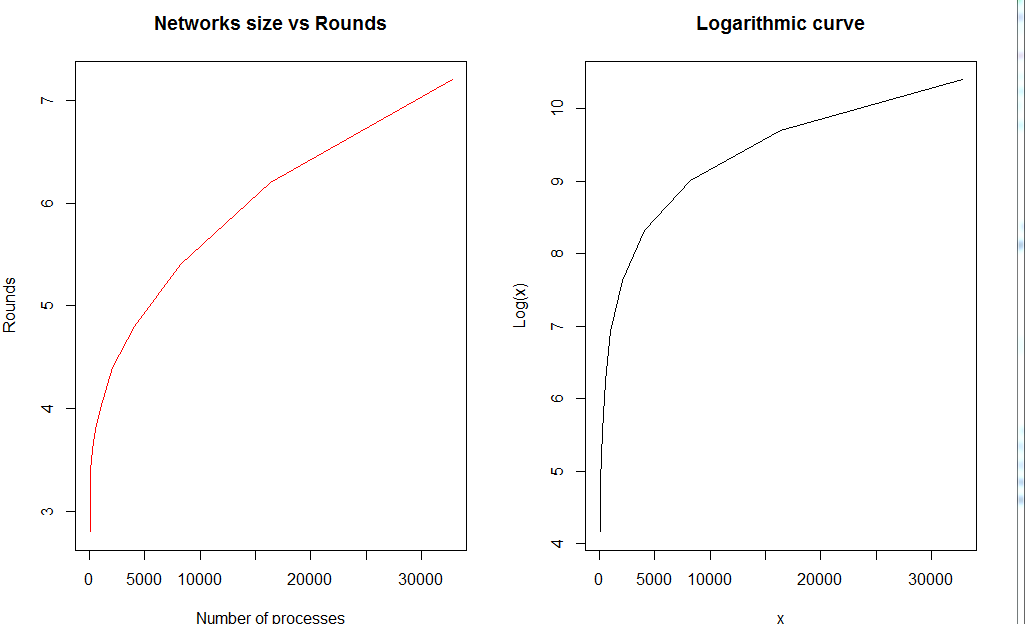
\includegraphics[width=1 \linewidth, height=5cm]{number_rounds.png} 
\caption{Rounds per execution}
\label{fig:rounds_execution}
\end{figure}

It is expected a progression in each round of the algorithm regarding the number of processes that finish the execution and become inactive. Once a processes finish the execution it output the final state (\textit{MIS} member or not). The progression of the algorithm can be seen in the figure \ref{fig:progression} for a network of 32768 processes. The blue line represents the number of processes that join the \textit{MIS}  per round and the red line shows the number of processes that are neighbours of some process that join the MIS. The figure \ref{fig:actives}, shows the total number of processes that are active in each round for the same topology. 

\begin{figure}[ht]
\centering
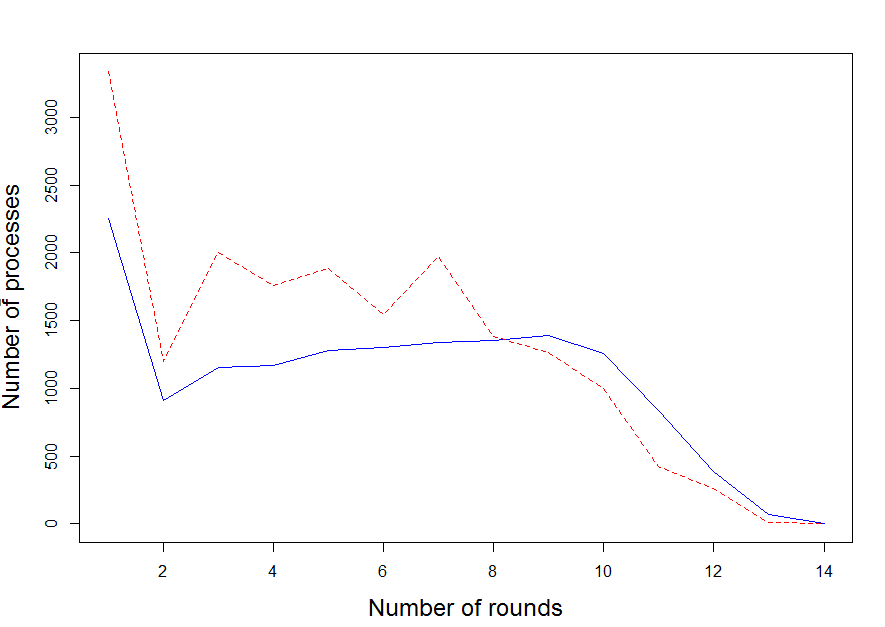
\includegraphics[width=0.7 \linewidth, height=5cm]{progress.PNG} 
\caption{Numbers of processes that finish the execution per round}
\label{fig:progression}
\end{figure}

\begin{figure}[ht]
\centering
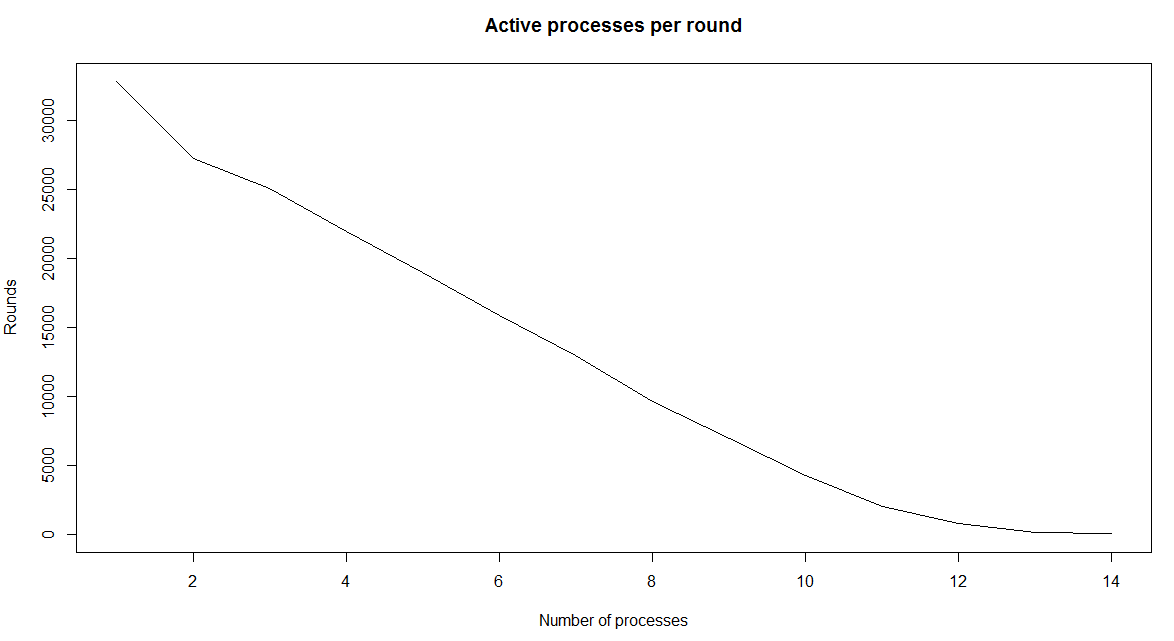
\includegraphics[width=0.7 \linewidth, height=5cm]{actives_round.PNG} 
\caption{Numbers of processes that finish the execution per round}
\label{fig:actives}
\end{figure}


\begin{figure}[ht]
\centering
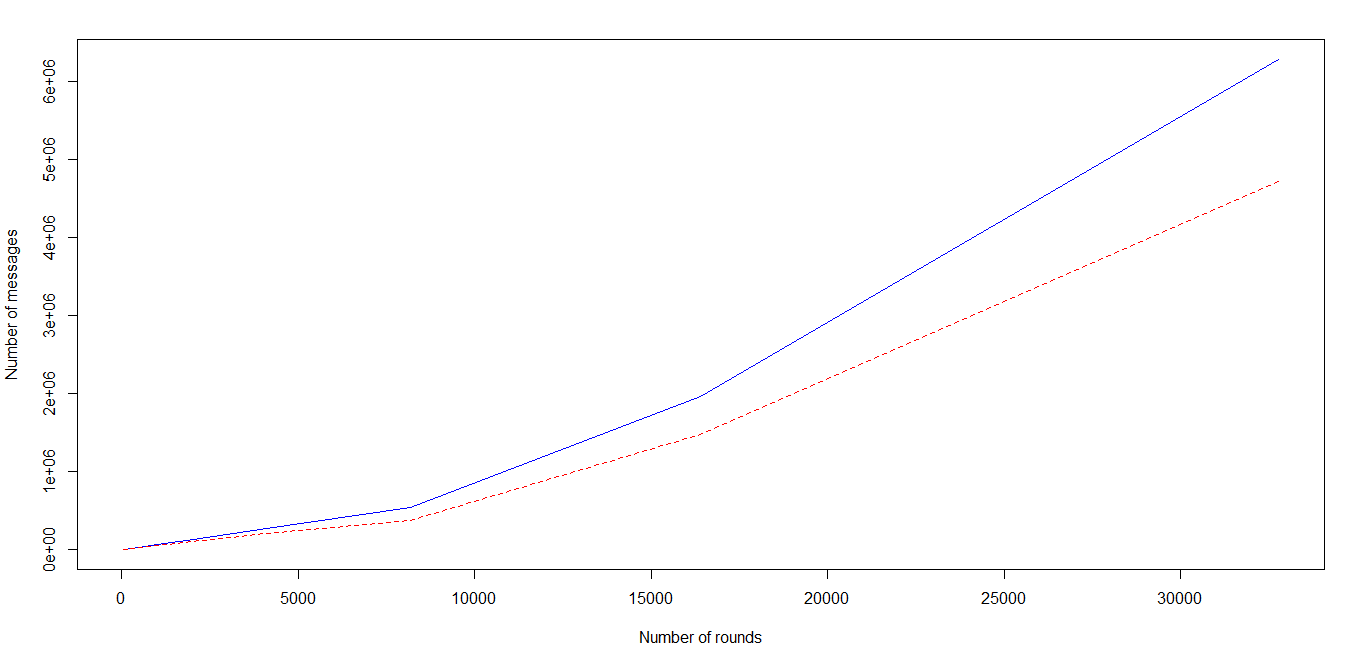
\includegraphics[width=0.7 \linewidth, height=5cm]{total_messages.PNG} 
\caption{Comparison between messages send for the protocol and the Global Synchronizer}
\label{fig:total_msg}
\end{figure}


 
\subsection{Evaluation of Synchronizers}

In this section ...

\subsection{Conclusions}

In this dissertation, the problem of finding the Maximal Independent Set in general graphs was studied. Distributed algorithms provide better time complexity than sequential algorithm. For distributed algorithm, it is assumed that the communication system is synchronous. In general, algorithms in synchronous system are easy to design and have lower complexity, therefore a distributed synchronous algorithm was implemented in order to analyse time and message complexity for the \textit{MIS} problem.

